\section{Simulations}

For all the simulations only a unit length $L_z = 1$ \si{\meter} of the cylinder was considered. Assuming that this is only one part of a longer cylinder with $L_\mathrm{total} \gg R$ also justifies the cylindrical symmetry assumption done previously.

The scalar fields of $\kappa$ and $S$ are determined by the equations:
\begin{equation}
    \kappa(r) = \kappa_0 + (\kappa_R - \kappa_0)\left(\frac{r}{R}\right)^2
    \label{eq:kappa_field}
\end{equation}
\begin{equation}
    S(r) = S_0\exp\left(-\frac{(r-r_0)^2}{\sigma^2}\right)
    \label{eq:S_field}
\end{equation}

There will be two other values of interest throughout the simulations. The first one is the total power from the heat source:
\begin{equation}
    P_\mathrm{tot} = \int_0^R S(r)2\pi r \mathrm{d}r
    \label{eq:ptot_source}
\end{equation}
that will be calculated nearly exactly using the python function \texttt{scipy.integrate.quad} and \autoref{eq:S_field}. The other value it will be compared to is the heat flux on the border of the cylinder:
\begin{equation}
    \Gamma_Q(R) = 2\pi Rj_Q(R)
    \label{eq:flux_border}
\end{equation}
calculated from the numerical value of $j_Q$. Both should also be multiplied by the length $L_z$ to give watts instead of watts per meter but we are considering units of length so this is \mbox{$L_z = 1$ \si{\meter}} and thus ignored.

\subsection{Constant heat source and thermal conductivity}
\label{sec:simu_constant}

The first set of simulations will be done considering an ideal case, as in \autoref{sec:solution_anal}. The heat source was chosen to be \(S(r) \equiv S_0 = 1000\) \si{\watt\per\cubic\meter} and the conductivity of the cylinder \(\kappa(r) \equiv \kappa_0 = 10^{-3}\) \si{\watt\per\meter\per\kelvin}. Taking \(\sigma = 10^{10}\) enlarges the spread of \(S\), allowing us to consider it constant between \(r=0\) and \(r=R\).

Using a small amount of mesh intervals (\(N=10\)), the temperature and heat flux were obtained, as shown in \autoref{fig:temperature_constant} and \autoref{fig:heat_constant} respectively. The analytical solution is plotted alongside the simulation data. We can see that the temperature gradient is higher at the edge of the cylinder than close to its center, as expected. The gradient is also 0 at \(r=0\) for the analytical solution, which is coherent with the symmetry of the system. The heat flux also remains very linear with respect to \(r\), except when close to the center. This will be discussed later. Close to the border of the cylinder (\(r=R\)), the simulations match the analytical solution quite closely. Closer to the center however, the uniform (equidistant in \(r\)) mesh remains a lot closer to the analytical solution, while the non-uniform mesh (equidistant in \(r^2\)) seems to become linear. However, the gradient does not become 0 at \(r=0\). This could be explained by the sparcity of mesh nodes close to the center, the first one being at \(r=0\) \si{\centi\meter} and the second one at \(r \approx 1.5\) \si{\centi\meter} for the non-uniform mesh, alongside the piecewise linear interpolating functions \(\Lambda_i\). A similar phenomenon can be seen in the heat flux, where the heat flux was calculated at the center of each interval.

\begin{figure}[h]
    \centering
    \begin{subfigure}{0.5\linewidth}
        \centering
        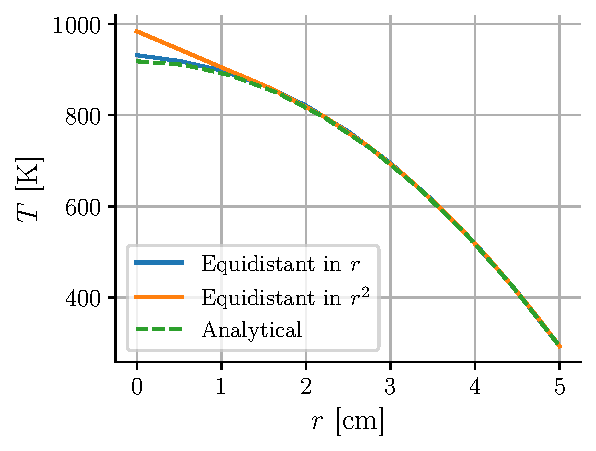
\includegraphics[width=\linewidth]{figures/temperature_constant.pdf}
        \caption{Temperature}
        \label{fig:temperature_constant}
    \end{subfigure}
    \begin{subfigure}{0.48\linewidth}
        \centering
        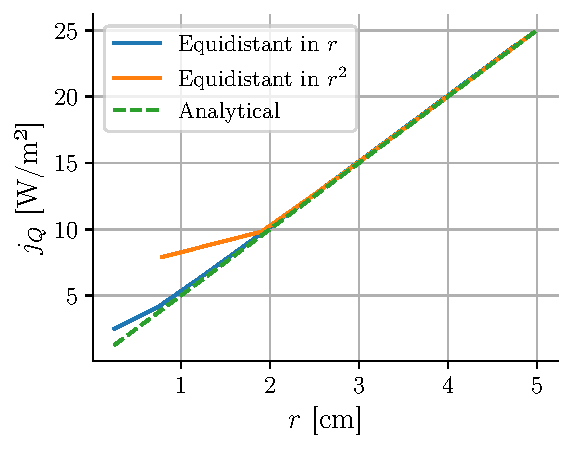
\includegraphics[width=\linewidth]{figures/heat_constant.pdf}
        \caption{Heat flux}
        \label{fig:heat_constant}
    \end{subfigure}
    \caption{Temperature and heat flux for \(N = 10\) mesh intervals, constant heat source \(S_0 = 1000\) \si{\watt\per\meter\cubed} and constant thermal conductivity \(\kappa = 10^{-3}\) \si{\watt\per\meter\per\kelvin}}
\end{figure}

The total power of the cylinder is given by \(\int_{0}^{R} S(r) 2\pi r \dd r = S_0 \pi R^2\) \si{\watt}, which should in theory be equal to the heat flux at the cylinder's border \(\Gamma_Q(R) = 2 \pi R j_Q(R)\) \si{\watt}. Using the heat flux computed inside the simulation closest to the border (\(r=R\)), the error on the global power balance is reported in \autoref{tab:error_global_power_constant}. One explanation for the difference comes from where the heat flux was measured: at the center of the final interval. Adjusting the total power to be calculated for \(r\) at the midpoint of the final interval yields much better results, lowering the relative deviation to 0.2\% for the uniform mesh and 0.06\% for the non-uniform mesh. It does then seem reasonable to assume that the global power balance is satisfied. The greater accuracy of the non-uniform mesh probably stems from the fact that the final midpoint is closer to \(R\) than the final midpoint of the uniform mesh.

\begin{table}[h]
    \centering
    \begin{tabulary}{\linewidth}{C|C C C C}
        \toprule
        & \(P_\textrm{tot}\) [\si{\watt}] & \(\Gamma_Q(R)\) [\si{\watt}] & Difference to \(P_\textrm{tot}(R)\) [\si{\watt}] & Relative deviation [\%] \\
        \midrule
        Uniform & 7.85 & 7.11 & 0.75 & 9.5 \% \\
        Non-uniform & 7.85 & 7.46 & 0.39 & 5.0 \% \\
        \bottomrule
    \end{tabulary}
    \caption{Error on global power balance for uniform and non-uniform mesh}
    \label{tab:error_global_power_constant}
\end{table}

Let's analyse the convergence of the finite element method under this system. Firstly, the error with respect to the analytical solution on the temperature at the center of the cylinder \(T(0)\) as a function of \(\frac{1}{N}\), where \(N\) is the number of mesh intervals, is shown in \autoref{fig:convergence_temp_N_constant}. We can see that the uniform mesh converges in order 2 while the non-uniform mesh converges in order 1. It is interesting to note that the actual order of convergence for the uniform mesh is 1.84, which we will consider to be order 2. The same error was also plotted as a function of the largest interval size in \autoref{fig:convergence_temp_interval_constant}. In this case, both mesh configurations converge in order 2. Again, the uniform mesh is closer to an order of 1.84, meaning that the temperature at the center converges faster with respect to the bigest interval size in the non-uniform case than the uniform case. For the same biggest interval size, the error with the non-uniform mesh is a bit smaller than the uniform mesh.

\begin{figure}[h]
    \centering
    \begin{subfigure}{0.48\linewidth}
        \centering
        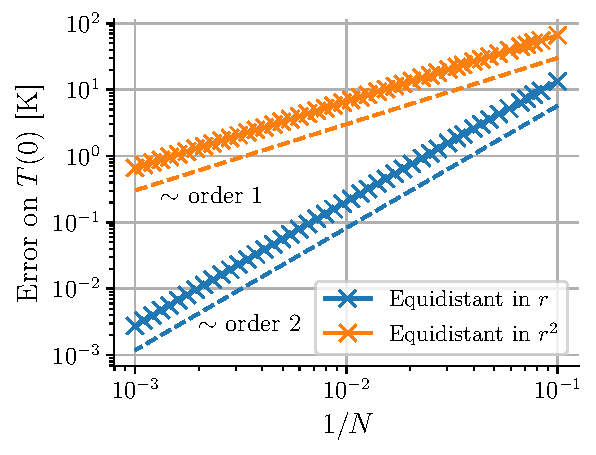
\includegraphics[width=\linewidth]{figures/convergence_temp_N_constant.pdf}
        \caption{Depending on mesh resolution}
        \label{fig:convergence_temp_N_constant}
    \end{subfigure}
    \begin{subfigure}{0.48\linewidth}
        \centering
        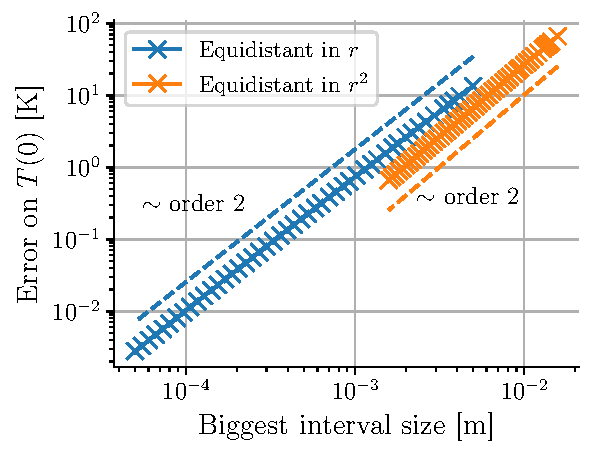
\includegraphics[width=\linewidth]{figures/convergence_temp_interval_constant.pdf}
        \caption{Depending on maximum interval length}
        \label{fig:convergence_temp_interval_constant}
    \end{subfigure}
    \caption{Convergence of temperature at the center of the cylinder, with constant heat source \(S_0 = 1000\) \si{\watt\per\meter\cubed} and constant thermal conductivity \(\kappa = 10^{-3}\) \si{\watt\per\meter\per\kelvin}}
    \label{fig:convergence_temp_constant}
\end{figure}

The convergence of the heat flux at the border of the cylinder \(j_Q(R)\) was also studied. \autoref{fig:convergence_heat_constant} shows that both mesh layouts converge with exactly order 1. The error with respect to the analytical solution is a bit lower for the non-uniform mesh than the uniform mesh. This could be explained by the higher point density close to \(R\) of the non-uniform mesh, yielding a better approximation of the temperature gradient close to \(R\). Similarly to the convergence of the heat flux at the border, the error on the global power balance decreases with order 1 with respect to \(\frac{1}{N}\), as shown in \autoref{fig:error_power_balance_constant}. The minimal error obtained here was for \(N = 1000\), which gave an error on the order of \(10^{-3}\), which isn't great but also not terrible. This means that for a very accurate simulation, if we want to conserve the global power balance, we would need a very fine mesh.

\begin{figure}[h]
    \begin{minipage}{0.47\linewidth}
        \centering
        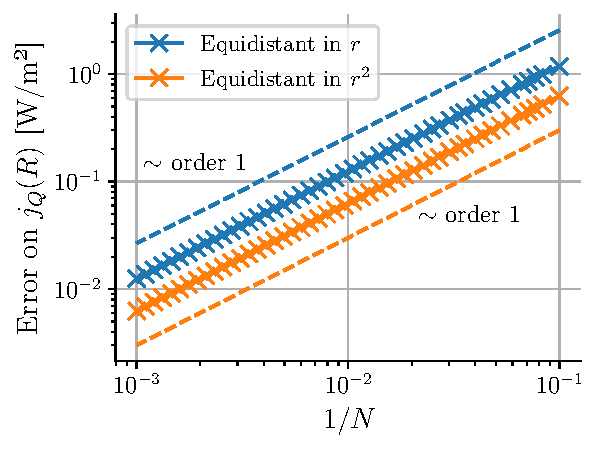
\includegraphics[width=\linewidth]{figures/convergence_heat_N_constant.pdf}
        \captionof{figure}{Convergence of heat flux at the cylinder's border \(r=R\), with constant heat source \(S_0 = 1000\) \si{\watt\per\meter\cubed} and constant thermal conductivity \(\kappa = 10^{-3}\) \si{\watt\per\meter\per\kelvin}}
        \label{fig:convergence_heat_constant}
    \end{minipage}
    \hspace{0.5cm}
    \begin{minipage}{0.5\linewidth}
        \centering
        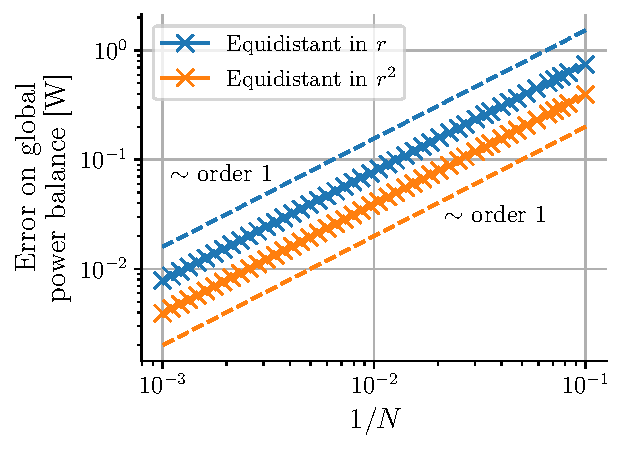
\includegraphics[width=\linewidth]{figures/convergence_power_balance_N_constant.pdf}
        \captionof{figure}{Error on global power balance \(|P_{\textrm{tot}} - \Gamma_Q(R)|\), with constant heat source \(S_0 = 1000\) \si{\watt\per\meter\cubed} and constant thermal conductivity \(\kappa = 10^{-3}\) \si{\watt\per\meter\per\kelvin}}
        \label{fig:error_power_balance_constant}
    \end{minipage}
\end{figure}

\subsection{Varying heat source and thermal conductivity}
We now keep $S_0 = 1000$ \si{\watt\per\cubic\meter} but take $r_0 = 0.03$ \si{\meter}, $\sigma = 0.005$ \si{\meter}, $\kappa_0 = 10^{-3}$ \si{\watt\per\meter\per\kelvin} and $\kappa_R = 10^{-5}$ \si{\watt\per\meter\per\kelvin}. This gives the conditions for our simulation using \autoref{eq:kappa_field} and \autoref{eq:S_field}. 

Similarly as in the previous part we take an equidistant mesh and a non-uniform one (but equidistant in $r^2$) and apply finite element analysis to find the values of $T$ and $j_Q$ at different points in the cylinder. The \autoref{fig:var_behavior} shows the results of this analysis for $N=10$ intervals as well as the result for a much larger $N=1000$ that is considered close enough to the physical result to be a point of comparison.
\begin{figure}[h]
    \centering
    \begin{subfigure}{0.48\linewidth}
        \centering
        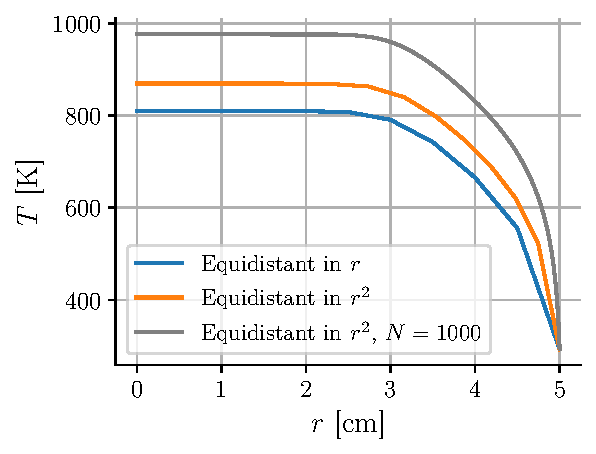
\includegraphics[width=\linewidth]{figures/var_T.pdf}
        \caption{Temperature in the cylinder}
        \label{fig:var_T}
    \end{subfigure}
    \begin{subfigure}{0.48\linewidth}
        \centering
        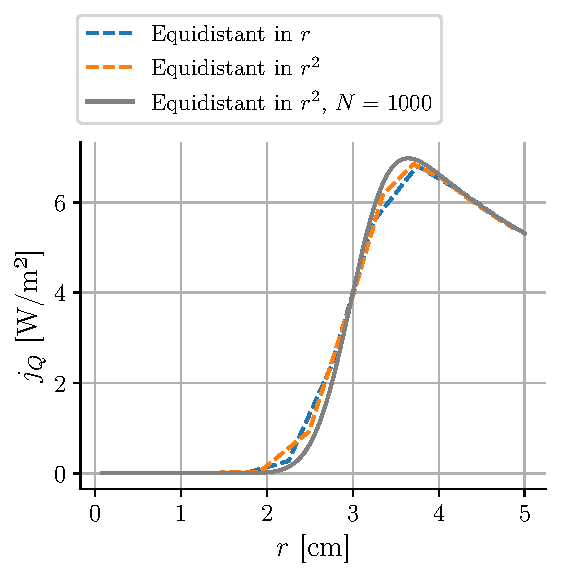
\includegraphics[width=\linewidth]{figures/var_j.pdf}
        \caption{Heat flux in the cylinder}
        \label{fig:var_j}
    \end{subfigure}
    \caption{Finite element analysis of a cylinder with heat source for $N = 10$ elements and $N=1000$ as a comparison}
    \label{fig:var_behavior}
\end{figure}

\autoref{fig:var_T} shows that the non-uniform mesh gives results significanly closer to the physical result (of $N=1000$). This better performance is also slightly visible in \autoref{fig:var_j} with curve for $r^2$ being closer to the physical one however this is much less significant. Overall both meshes give the right behavior with a constant temperature almost up to $r_0$ corresponding to the peak of the heat source. The peak of the heat source also seems to be the point where the convexity of $j_Q(r)$ changes in \autoref{fig:var_j}. This two indicators correspond to our intuition that the circular peak of heat source around the cylinder will have inside of it a temperature maintained constant by an equilibrium of heat produced and heat diffused away when outside of this peak source we should get closer to the outside temperature. It is of course logical that the temperature is greater inside the cylinder at equilibrium since it produces energy. The change of convexity in $j_Q(r)$ also can be explained by the fact that beyond the peak of the source the section of the cylinder increasing in $r^2$ will reduce the contribution of the source.

The values of $P_\mathrm{tot}$ and $\Gamma_Q(R)$ for the uniform and non-uniform mesh in this case of a non-homogeneous cylinder are given in \autoref{tab:error_power_var} with their difference and the relative deviation.
\begin{table}[H]
    \centering
    \begin{tabulary}{\linewidth}{C|C C C C}
        \toprule
        & \(P_\textrm{tot}\) [\si{\watt}] & \(\Gamma_Q(R)\) [\si{\watt}] & Difference to \(P_\textrm{tot}(R)\) [\si{\watt}] & Relative deviation [\%] \\
        \midrule
        Uniform & 1.67 & 1.76 & 0.09 & 5.3 \% \\
        Non-uniform & 1.67 & 1.71 & 0.03 & 2.1 \% \\
        \bottomrule
    \end{tabulary}
    \caption{Error on global power balance for uniform and non-uniform mesh in non-homogeneous cylinder}
    \label{tab:error_power_var}
\end{table}

We have from \autoref{tab:error_power_var} that both methods are quite precise here giving slightly smaller errors than in the previous part and with the non-uniform equidistant in $r^2$ mesh still being the most precise of the two indicating once again that it is a more adapted mesh. Despite the very low number of intervals $N=10$ both this error and the behavior of the numerical simulation are coherent with the theory and our intuition which indicates that finite element analysis respects well the physical reality of this system.


Now that the general behavior of our simulation has been confirmed to be consistent with the theory we want to anaylse its convergence and the converged values. In that purpose simulations with 500 to 5000 intervals were run and the values of the temperature at the center $T(0)$, the flux at the border $j_Q(R)$ and the error on the balance of power are shown in \autoref{fig:var_convergence} according to $1/N$. The power of $1/N$ was chosen to have the points align which gives the order of convergence for each value.
\begin{figure}[H]
    \centering
    \begin{subfigure}{0.48\linewidth}
        \centering
        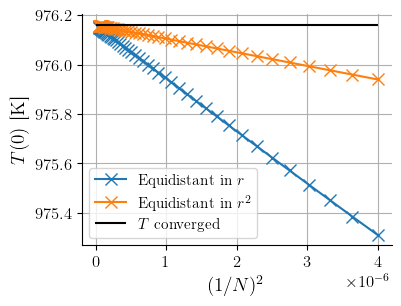
\includegraphics[width=\linewidth]{figures/var_conv_T.png}
        \caption{Convergence of temperature}
        \label{fig:var_conv_T}
    \end{subfigure}
    \begin{subfigure}{0.48\linewidth}
        \centering
        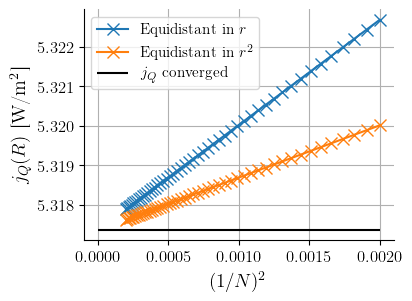
\includegraphics[width=\linewidth]{figures/var_conv_j.png}
        \caption{Convergence of heat flux}
        \label{fig:var_conv_j}
    \end{subfigure}
    \begin{subfigure}{0.48\linewidth}
        \centering
        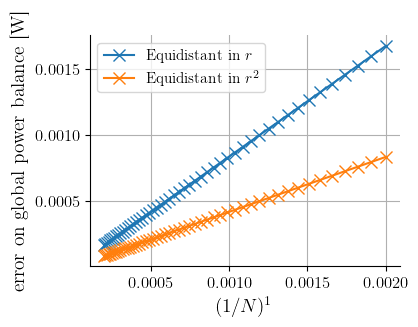
\includegraphics[width=\linewidth]{figures/var_conv_error.png}
        \caption{Convergence of error on power balance}
        \label{fig:var_conv_error}
    \end{subfigure}
    \caption{Convergence analysis of the temperature, heat flux and error on the global power balance according to the number $N$ of intervals in the mesh}
    \label{fig:var_convergence}
\end{figure}

We see in \autoref{fig:var_conv_T} that the value for $T(0)$ converges in order 2 for both the uniform and non-uniform mesh. For $j_Q(R)$ and the error on power balance the convergence is of order 1 for both meshes. It is then clearly illustrated that both meshes converge in the same order for all the variables considered however it is interesting to note that every time the one equidistant in $r^2$ is again performing better. In \autoref{fig:var_conv_T} and \autoref{fig:var_conv_j} this corresponds to it being consistently closer to the converged value and for \autoref{fig:var_conv_error} to it being closer to 0. Indeed we know physically that the power balance should be 0 to have conservation of energy so this is the analytical value the simulations converge to.

For the converged values of \autoref{fig:var_conv_T} and \autoref{fig:var_conv_j} we took a polynomial of order the order of convergence and fitted it to the data and $1/N$. Taking the value of this polynomial at $0$ gives the converged value. This linear fit was done for both the datas from the uniform and non-uniform meshes but since the non-uniform has been consistently analysed to be performing better and the relative deviation was at most of $10^{-4}$\% between the two only the value for the non-uniform one was kept. We found for $T_\mathrm{conv}(0) = 976.16$ \si{\kelvin} and $j_{Q,\mathrm{conv}}(R) = 5.32$ \si{\watt\per\meter\squared} which is very close to the values seen in the more precise simulation in \autoref{fig:var_behavior} so our analysis was consistent. We can do a final balance of power using this new converged value of $j_Q$ and find that: \hbox{$|P_\mathrm{tot} - \Gamma_{Q,\mathrm{conv}}(R)| = 4.55 \times 10^{-7}$ \si{\watt}} so with this convergence value the energy is very well conserved.

\subsection{Changing integration method}

The integration method for initialising the matrix elements can also be changed. Until now, the midpoint rule was used. The implementation was changed to allow a mix of the trapezoidal rule and midpoint rule, with a parameter \(p\) setting the weight of each method. Setting \(p = 0\) means only using the midpoint rule and \(p = 1\) is only the trapezoidal rule. The formula for integration then becomes:
\begin{equation}
    \int_{x_k}^{x_{k+1}} f(x) \dd x \approx h_k \left[ p \frac{f(x_k) + f(x_{k+1})}{2} + (1-p) f \left( \frac{x_k + x_{k+1}}{2} \right) \right]
\end{equation}
Using the same configuration as in \autoref{sec:simu_constant}, we obtain a temperature and heat flux as shown in \autoref{fig:temperature_exact} and \autoref{fig:heat_exact}. A very interesting phenomenon occured: in both cases, the simulations match the analytical solution exactly at the mesh nodes, while only differing in between nodes due to the linear interpolation! This is because \textbf{FEUR MARTIN OSKOUR}.

\begin{figure}[h]
    \centering
    \begin{subfigure}{0.5\linewidth}
        \centering
        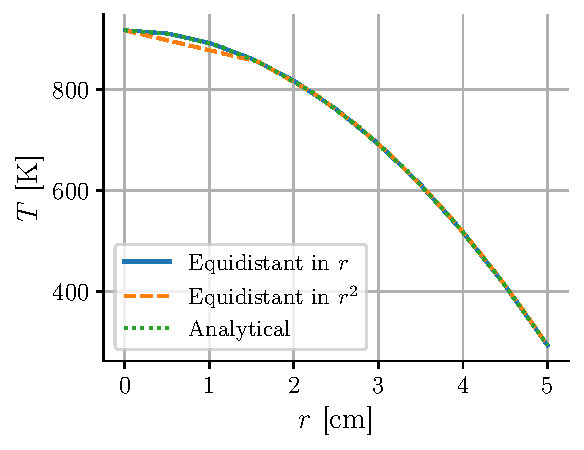
\includegraphics[width=\linewidth]{figures/temperature_exact.pdf}
        \caption{Temperature}
        \label{fig:temperature_exact}
    \end{subfigure}
    \begin{subfigure}{0.48\linewidth}
        \centering
        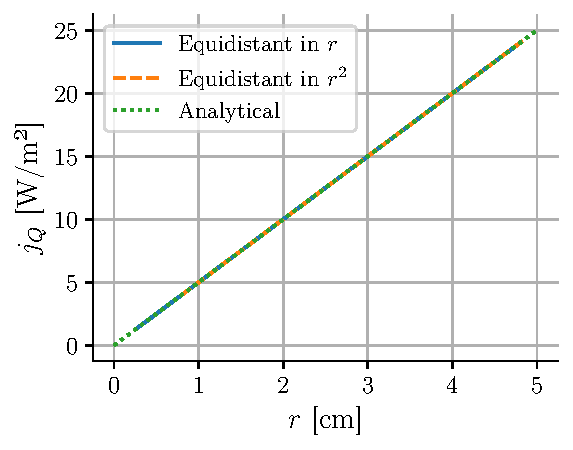
\includegraphics[width=\linewidth]{figures/heat_exact.pdf}
        \caption{Heat flux}
        \label{fig:heat_exact}
    \end{subfigure}
    \caption{Temperature and heat flux for \(N = 10\) mesh intervals, constant heat source \(S_0 = 1000\) \si{\watt\per\meter\cubed} and constant thermal conductivity \(\kappa = 10^{-3}\) \si{\watt\per\meter\per\kelvin}}
\end{figure}
